% ============================================================================
%  Project Report — Template Format
%  Deep Learning-Based Time-of-Day Estimation from Sky Images
%  and EXIF Calendar Dates
% ============================================================================
\documentclass[9pt, a4paper, twocolumn]{article}

% ── Packages ────────────────────────────────────────────────────────────────
\usepackage[utf8]{inputenc}
\usepackage[T1]{fontenc}
\usepackage{mathptmx}            % Serif font similar to Cambria
\usepackage[left=2cm, right=2cm, top=2.5cm, bottom=2.5cm]{geometry}
\usepackage{amsmath, amssymb}
\usepackage{graphicx}
\usepackage{booktabs}
\usepackage{array}
\usepackage{float}
\usepackage{hyperref}
\usepackage[english]{babel}
\usepackage{setspace}
\usepackage{titlesec}
\usepackage{enumitem}
\usepackage{caption}
\usepackage{fancyhdr}
\usepackage{multicol}
\usepackage{tabularx}

% ── Spacing ─────────────────────────────────────────────────────────────────
\singlespacing
\setlength{\parindent}{0pt}
\setlength{\parskip}{5pt}
\setlength{\columnsep}{0.6cm}

% ── Section formatting (bold, 9pt) ─────────────────────────────────────────
\titleformat{\section}
  {\normalsize\bfseries}{\thesection.}{0.5em}{}
\titleformat{\subsection}
  {\normalsize\bfseries}{\thesubsection.}{0.5em}{}
\titlespacing*{\section}{0pt}{10pt}{5pt}
\titlespacing*{\subsection}{0pt}{8pt}{4pt}
\titleformat{\subsubsection}
  {\normalsize\itshape}{\thesubsubsection.}{0.5em}{}
\titlespacing*{\subsubsection}{0pt}{6pt}{3pt}

% ── Caption formatting ─────────────────────────────────────────────────────
\captionsetup{font=small, labelfont=bf, skip=5pt}

% ── Hyperref setup ─────────────────────────────────────────────────────────
\hypersetup{
    colorlinks=true,
    linkcolor=black,
    citecolor=black,
    urlcolor=blue
}

% ============================================================================
\begin{document}

% ── Title (14pt, left-aligned) ─────────────────────────────────────────────
\twocolumn[
\begin{@twocolumnfalse}
\begin{flushleft}
{\fontsize{14}{17}\selectfont\bfseries
Deep Learning-Based Time-of-Day Estimation from Sky Images and EXIF Calendar Dates}
\vspace{8pt}

{\normalsize
Alk\i m G\"onen\c{c} Efe$^{1}$, Sarp S\"unb\"ul$^{1}$, Damla Parlaky\i ld\i z$^{1}$}
\vspace{4pt}

{\small\itshape
$^{1}$Department of Computer Engineering, İzmir Katip Çelebi University, İzmir, Türkiye}
\vspace{4pt}

\rule{\textwidth}{0.4pt}

\vspace{4pt}
{\small\bfseries Abstract}
\vspace{2pt}

{\small
Automated image organization systems in modern digital galleries frequently rely on simplistic brightness-based heuristics to classify outdoor photographs by time of day, leading to systematic misclassifications under artificial lighting and overcast conditions. This paper presents a hybrid deep learning framework that estimates the exact time of capture from a single sky image by fusing visual features extracted by a ConvNeXt-Tiny convolutional backbone with cyclically encoded EXIF calendar metadata. The proposed architecture integrates 77-dimensional handcrafted photometric descriptors---including color-space statistics, sky-region luminance gradients, and edge density measures---with learned deep representations through a metadata fusion multilayer perceptron. A cyclic sine--cosine target encoding is employed to model the circular nature of the 24-hour clock, ensuring continuity at the midnight boundary. The training pipeline incorporates Mixup data augmentation, label noise injection, cosine annealing scheduling, and weighted sampling to address class imbalance across temporal bins. Additionally, a parallel MATLAB-based pipeline utilizing SqueezeNet with Random Forest and Support Vector Regression baselines is developed for comparative analysis. Five-fold cross-validation is used for model evaluation.
}
\vspace{4pt}

{\small\bfseries Keywords:} {\small time-of-day estimation, convolutional neural networks, ConvNeXt, EXIF metadata, cyclic regression, sky image analysis, feature fusion}

\vspace{6pt}
\rule{\textwidth}{0.4pt}
\vspace{12pt}
\end{flushleft}
\end{@twocolumnfalse}
]

% ========================================================================
%  1. INTRODUCTION
% ========================================================================
\section{Introduction}

The estimation of time of day from a single outdoor photograph is a challenging problem at the intersection of computer vision, digital image processing, and environmental sensing. Modern mobile operating systems and cloud storage services attempt to semantically organize landscape photographs, yet their algorithms frequently produce unreliable temporal classifications due to an over-reliance on simplistic brightness metrics [1].

Two principal failure modes motivate this research. First, nighttime images containing strong artificial light sources---such as street lamps, stadium floodlights, or illuminated building facades---are routinely misclassified as ``Daylight'' or ``Sunny'' because high localized luminance inflates the average pixel intensity. Second, midday photographs captured under heavy cloud cover or in deeply shaded areas are often mislabeled as ``Night'' or ``Twilight'' due to globally suppressed light levels that mislead intensity-based classifiers.

These systematic errors underscore a fundamental limitation: average brightness alone is an insufficient proxy for solar position. A robust estimator must instead analyze complex visual cues---shadow geometry, atmospheric color temperature shifts from blue to warm orange, sky gradient profiles, and textural patterns in cloud formations---to replicate the human cognitive ability to distinguish natural from artificial illumination [2].

A foundational study by Lalonde et al. [1] introduced the concept of utilizing ``weak cues'' extracted from various image segments---the sky region, vertical surfaces, and the ground plane---to estimate sun position and visibility. Their work demonstrated that while any single visual feature in isolation may be uninformative, the probabilistic integration of multiple complementary cues leads to a robust estimate of the sky dome's appearance. The present project adopts this multi-cue philosophy by analyzing both sky gradients and color temperatures to identify solar characteristics, extending the concept to a learned feature-fusion framework.

The ``Photo Sundial'' system proposed by Wu et al. [3] explicitly addressed the issue of unreliable EXIF timestamps in consumer photography. The authors developed a framework that utilizes astronomical theory, linking the sun's apparent position and the camera's viewing direction to calculate the exact time of capture. This study is particularly relevant to the forensic image analysis motivation of the present work and the correction of mislabeled gallery metadata.

Recent advancements by Hold-Geoffroy et al. [2] shifted the paradigm from analytical parametric models to learned high dynamic range (HDR) sky representations. They highlighted the limitations of traditional parametric sky models (e.g., the Hosek--Wilkie model) in representing non-clear-sky conditions such as overcast or partially cloudy weather. By training a convolutional neural network (CNN) to learn sky representations directly from data, they achieved superior results under diverse meteorological conditions.

Unlike previous studies that often treat the date of capture as a static categorical label or ignore it entirely, this project integrates the calendar date directly into the model's feature vector through cyclic encoding. This allows the system to distinguish between identical lighting conditions that occur at different solar angles during the winter and summer solstices. The purpose of this study is to develop a hybrid deep learning framework that transcends simple luminance metrics, combining visual feature extraction with temporal metadata integration for robust, continuous time-of-day regression from consumer sky photographs.


% ========================================================================
%  2. MATERIALS AND METHODS
% ========================================================================
\section{Materials and Methods}

This section describes the complete pipeline for time-of-day estimation, encompassing data collection, preprocessing, feature extraction, model architecture, training strategy, and evaluation protocol. Two parallel implementations were developed: a primary Python/PyTorch pipeline centered on a ConvNeXt backbone, and a secondary MATLAB pipeline utilizing SqueezeNet with classical machine learning baselines.

\subsection{Dataset Construction and Preprocessing}

The dataset comprises outdoor sky photographs collected from the personal galleries of the research team members using consumer-grade smartphone cameras. Each image is required to contain visible sky content and to carry valid EXIF metadata including the \texttt{DateTimeOriginal} tag. Supported image formats include JPEG, PNG, HEIC, and DNG (raw).

For each image, the following metadata fields are extracted from the EXIF header using a dual-library strategy (\texttt{exifread} as the primary parser, with Pillow as a fallback): (i) capture time, parsed from \texttt{DateTimeOriginal}, \texttt{DateTime}, or \texttt{DateTimeDigitized} tags and converted to minutes since midnight ($t \in [0, 1440)$); (ii) calendar date (month, day, year) used to compute the day of year ($d \in [1, 366]$); and (iii) GPS coordinates (latitude and longitude), normalized to $[-1, 1]$. Images lacking valid temporal EXIF data are excluded.

All images are preprocessed through a resolution-standardization pipeline. Original images are downscaled to a maximum dimension of 512 pixels using Lanczos resampling while preserving the aspect ratio. Downscaled images are saved as JPEG files at 90\% quality with EXIF metadata preserved using the \texttt{piexif} library. At training time, images are further processed through a letterbox resize to a fixed $512 \times 512$ canvas with black padding and normalized using ImageNet statistics ($\mu = [0.485, 0.456, 0.406]$, $\sigma = [0.229, 0.224, 0.225]$), a standard preprocessing scheme for deep convolutional neural networks trained on large-scale datasets [7,8]. For the MATLAB pipeline, images are resized to $224 \times 224$ pixels.

\subsection{Feature Engineering}

\subsubsection{Handcrafted Photometric Features}

A comprehensive set of 77 handcrafted image features is extracted from each photograph. These features are organized as follows: RGB channel statistics (mean and standard deviation per channel, 6 dims), HSV channel statistics (6 dims), CIELAB channel statistics normalized (6 dims), RGB histograms with 8 bins per channel (24 dims), HSV histograms with 8 bins per channel (24 dims), sky-region luminance computed as mean and standard deviation of the value channel in the top third of the frame (2 dims), vertical luminance gradient (1 dim), color temperature proxy as the R/B channel ratio (1 dim), global luminance with mean, standard deviation, and entropy (3 dims), saturation statistics (2 dims), Canny edge density (1 dim), and Laplacian variance as a cloud texture measure (1 dim).

Color space conversions are performed using the \texttt{scikit-image} library. Edge detection is implemented using the Canny operator [9], which provides robust gradient-based edge localization under varying noise conditions.

\subsubsection{Calendar Metadata Encoding}

Temporal metadata is encoded using cyclic trigonometric transformations to preserve circular continuity:

\begin{equation}
{
\renewcommand{\arraystretch}{1.4}
\mathbf{m}_{\text{cal}} =
\begin{bmatrix}
\sin\!\left(\frac{2\pi \cdot \text{month}}{12}\right),
\cos\!\left(\frac{2\pi \cdot \text{month}}{12}\right), \\
\sin\!\left(\frac{2\pi \cdot \text{doy}}{365.25}\right),
\cos\!\left(\frac{2\pi \cdot \text{doy}}{365.25}\right), \\
\frac{\text{lat}}{90},
\frac{\text{lon}}{180}
\end{bmatrix}^T
}
\end{equation}

This encoding ensures that December and January are treated as adjacent months and avoids discontinuities inherent in linear representations of periodic variables. Such sine--cosine encodings are a standard technique for representing cyclical features in machine learning. The complete metadata vector has dimensionality $d_{\text{meta}} = 6 + 77 = 83$ when image features are enabled.

\subsection{Target Encoding}

The regression target is encoded as a unit-circle representation to respect the circular topology of the 24-hour clock:

\begin{equation}
\mathbf{y} = \left[\sin\!\left(\frac{2\pi t}{1440}\right),\;
\cos\!\left(\frac{2\pi t}{1440}\right)\right]^T
\end{equation}

where $t$ is the time in minutes since midnight. Decoding is performed via $\hat{t} = \frac{\text{atan2}(\hat{y}_{\sin}, \hat{y}_{\cos}) \bmod 2\pi}{2\pi} \times 1440$. This encoding eliminates discontinuities at midnight and ensures smooth gradients across the temporal boundary.

\subsection{Python Implementation: ConvNeXt with Metadata Fusion}

The primary Python/PyTorch pipeline is built around a ConvNeXt-Tiny backbone pretrained on ImageNet-1K [7]. Figure~\ref{fig:python_arch} illustrates the overall architecture.

\begin{figure}[H]
  \centering
  
\includegraphics[width=0.8\linewidth]{python_arch.png}
  \caption{Python pipeline: ConvNeXt-Tiny backbone with metadata fusion MLP.}
  \label{fig:python_arch}
\end{figure}

\subsubsection{Model Architecture}

The ConvNeXt-Tiny backbone [4] produces a 768-dimensional feature vector after global average pooling. All stages up to \texttt{features.4} are frozen during training. The 768-dimensional image feature is concatenated with the 83-dimensional metadata vector to form an 851-dimensional input to a three-layer MLP with hidden dimension 384, GELU activations, layer normalization, and dropout (rate 0.156):

\begin{equation}
\begin{aligned}
\mathbf{h}_1 &= \text{Drop}\!\left(\text{GELU}\!\left(
    \text{LN}\!\left(\mathbf{W}_1 [\mathbf{f}_{\text{img}};
    \mathbf{m}] + \mathbf{b}_1\right)\right)\right) \\
\mathbf{h}_2 &= \text{Drop}\!\left(\text{GELU}\!\left(
    \text{LN}\!\left(\mathbf{W}_2 \mathbf{h}_1 +
    \mathbf{b}_2\right)\right)\right) \\
\hat{\mathbf{y}} &= \mathbf{W}_3 \mathbf{h}_2 + \mathbf{b}_3
\end{aligned}
\end{equation}

\subsubsection{Loss Function and Evaluation Metric}

The model is trained with MSE loss on the sine--cosine encoded targets:

\begin{equation}
\mathcal{L} = \frac{1}{N} \sum_{i=1}^{N}
    \left\| \hat{\mathbf{y}}_i - \mathbf{y}_i \right\|_2^2
\end{equation}

The primary evaluation metric is cyclic MAE in minutes:

\begin{equation}
\text{MAE}_{\text{cyc}} = \frac{1}{N} \sum_{i=1}^{N}
    \min\!\left(|\hat{t}_i - t_i|,\; 1440 - |\hat{t}_i - t_i|\right)
\end{equation}

\subsubsection{Training and Optimization}

A heavy augmentation regime is employed: random resized crop, horizontal flipping, RandAugment [10], random erasing [11], and Mixup [12]. The optimizer is 8-bit AdamW [5] combined with cosine annealing [14]. Hyperparameters are found via Optuna [6] Bayesian search over 15 trials. A weighted random sampler handles the non-uniform distribution of capture times [15].

\subsubsection{Ensemble Inference}

Predictions from all five fold checkpoints are averaged in sine--cosine space and re-normalized onto the unit circle:

\begin{equation}
\hat{\mathbf{y}}_{\text{ens}} = \frac{1}{K} \sum_{k=1}^{K}
    \hat{\mathbf{y}}_k, \qquad
\tilde{\mathbf{y}} = \frac{\hat{\mathbf{y}}_{\text{ens}}}
    {\|\hat{\mathbf{y}}_{\text{ens}}\|_2}
\end{equation}

This ensemble strategy reduces prediction variance across random fold splits [16].

\subsection{MATLAB Implementation: SqueezeNet with Classical Baselines}

The MATLAB pipeline provides a parallel, computationally lighter implementation using MATLAB's Deep Learning Toolbox. Figure~\ref{fig:matlab_arch} shows the multi-input architecture.

\begin{figure}[H]
  \centering
  
\includegraphics[width=0.8\linewidth]{matlab_arch.png}
  \caption{MATLAB pipeline: multi-input SqueezeNet with a date encoding branch.}
  \label{fig:matlab_arch}
\end{figure}

\subsubsection{Multi-Input CNN Architecture}

The image branch uses SqueezeNet [17] with fire modules fire1--fire6 frozen and fire7--fire9 fine-tuned, producing a 512-dimensional feature vector. A parallel date branch encodes the four cyclic calendar features through two fully connected layers, yielding a 64-dimensional vector. Both branches are concatenated and passed through the following head:
\begin{itemize}[noitemsep,topsep=2pt]
  \item FC(256) $\to$ BN $\to$ ReLU $\to$ Dropout(0.4)
  \item FC(64) $\to$ ReLU $\to$ FC(1) $\to$ RegressionLayer
\end{itemize}
The network is trained for 30 epochs using Adam with MSE loss on time in fractional hours.

\subsubsection{Classical Baselines}

Two classical baselines are trained on the 145-dimensional handcrafted feature vector plus the 4-dimensional date encoding. The \textbf{Random Forest} uses 100 decision trees via \texttt{TreeBagger} [18]. The \textbf{Support Vector Regressor} uses an RBF kernel via \texttt{fitrsvm} with automatic feature scaling [19]. Both baselines provide lower-bound reference points for the CNN.

\subsection{Cross-Validation Protocol}

Both pipelines use 5-fold cross-validation with stratified random shuffling and a fixed seed (42). This provides robust performance estimation and reduces variance from a single train-test split [20].

% ========================================================================
%  3. EXPERIMENTAL SETUP
% ========================================================================
\section{Experimental Setup}

\subsection{Dataset}

The dataset contains 2,483 outdoor sky photographs collected by the research team using consumer smartphones and a mirrorless camera. Images span diverse conditions including dawn, midday, dusk, overcast skies, and artificial-light scenes, covering captures from 2023 to 2026. Table~\ref{tab:dataset} summarizes the key statistics.

\begin{table}[H]
\centering
\footnotesize
\caption{Dataset summary.}
\label{tab:dataset}
\begin{tabular}{lc}
\toprule
\textbf{Property} & \textbf{Value} \\
\midrule
Total images        & 2,483 \\
Formats             & JPEG, HEIC, PNG, DNG \\
Time span           & 03:00--23:25 \\
Capture period      & 2023--2026 \\
Cross-val folds     & 5 \\
Python resolution   & $512\times512$ (letterboxed) \\
MATLAB resolution   & $224\times224$ \\
\bottomrule
\end{tabular}
\end{table}

Figures~\ref{fig:dataset_temporal} and~\ref{fig:dataset_calendar} show the temporal and calendar distributions of the dataset, respectively.

\begin{figure}[H]
  \centering
  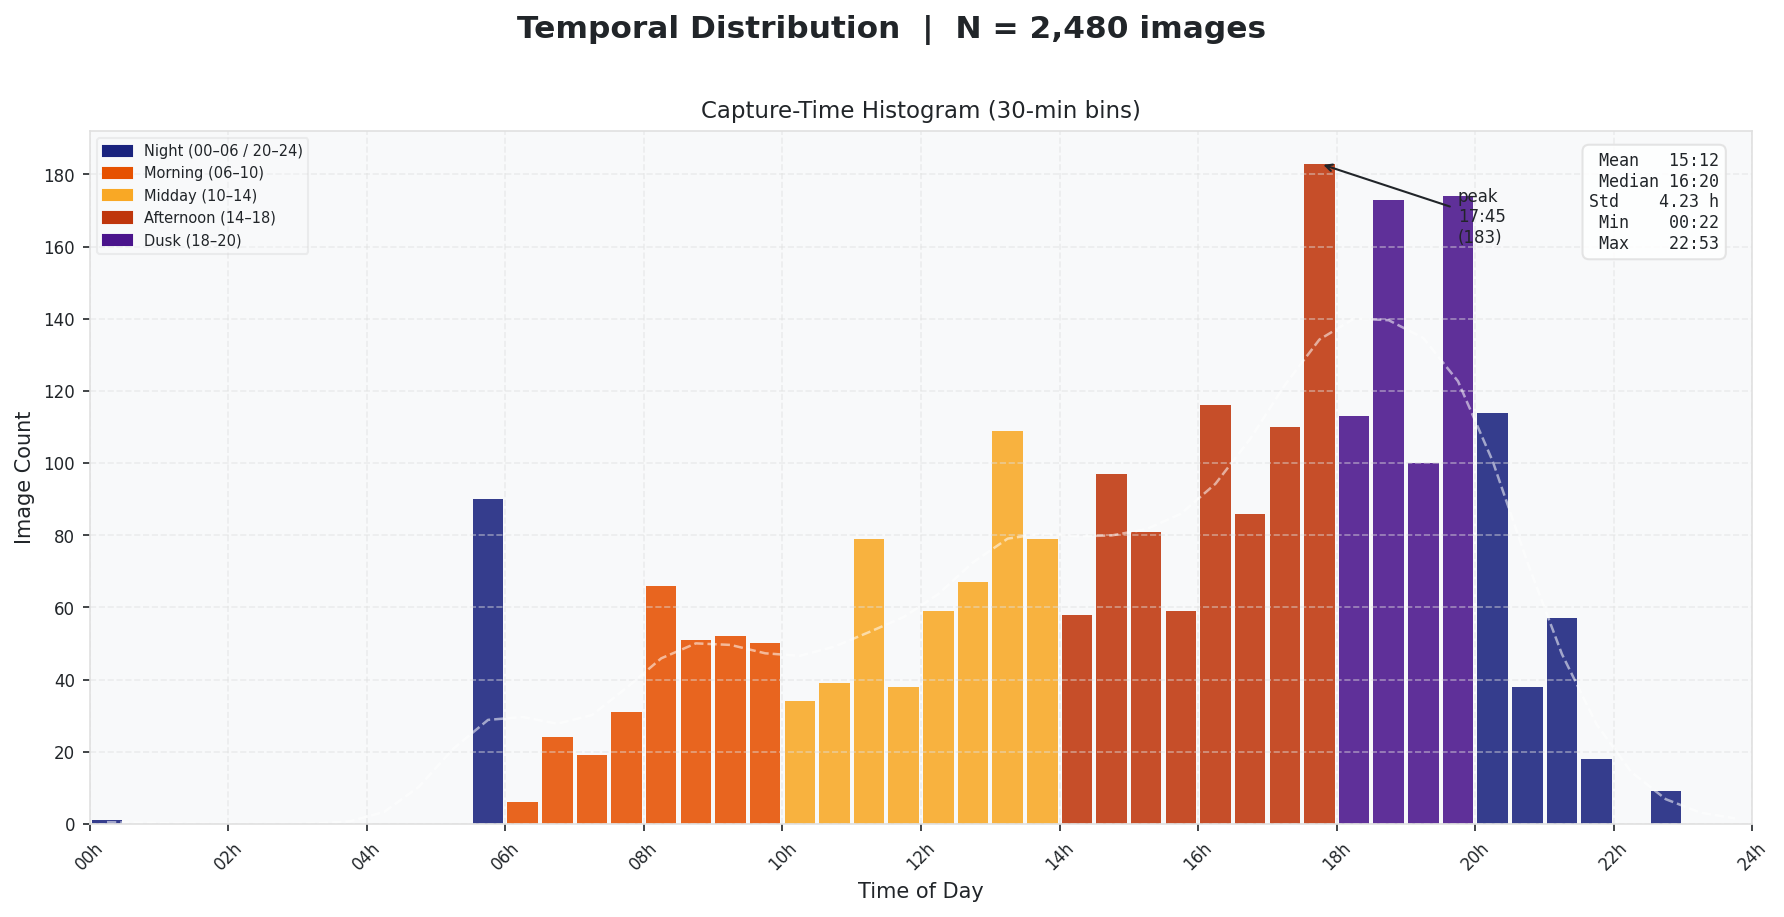
\includegraphics[width=0.75\linewidth]{dataset_report_p1_temporal.png}
  \caption{Temporal distribution of capture times across the dataset.}
  \label{fig:dataset_temporal}
\end{figure}

\begin{figure}[H]
  \centering
  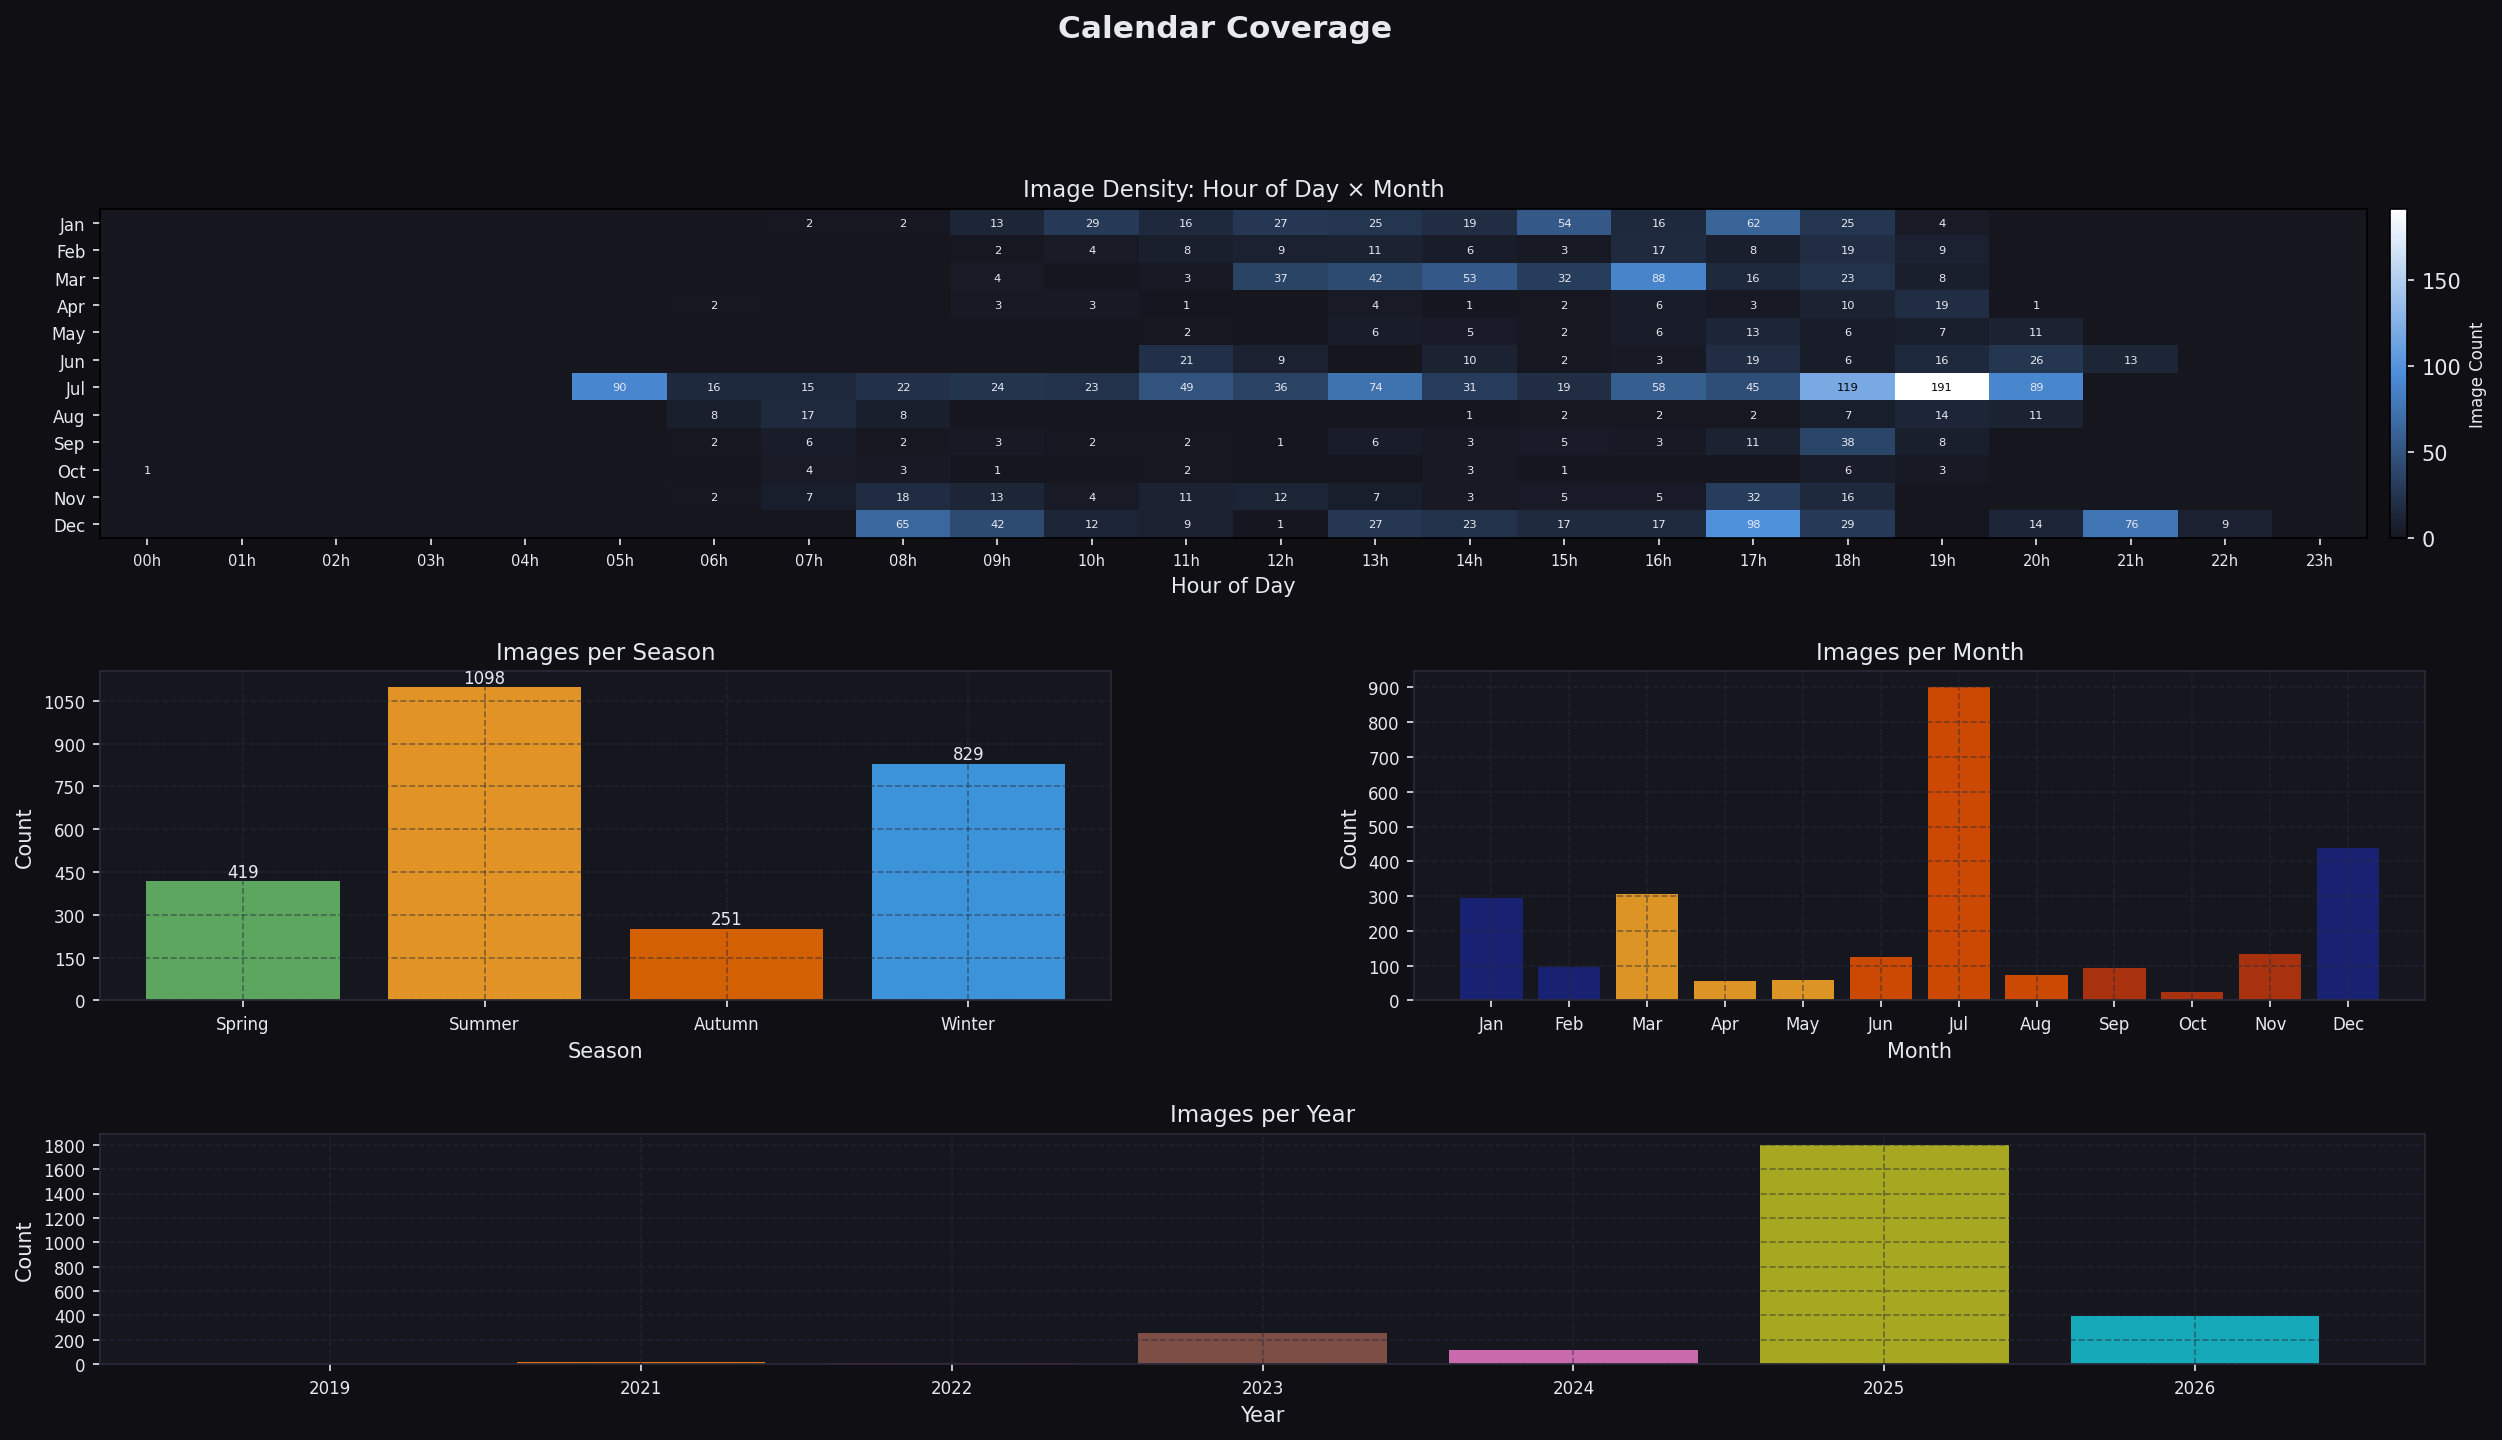
\includegraphics[width=0.75\linewidth]{dataset_report_p2_calendar.png}
  \caption{Calendar distribution of captures across months and seasons.}
  \label{fig:dataset_calendar}
\end{figure}

\begin{figure}[H]
  \centering
  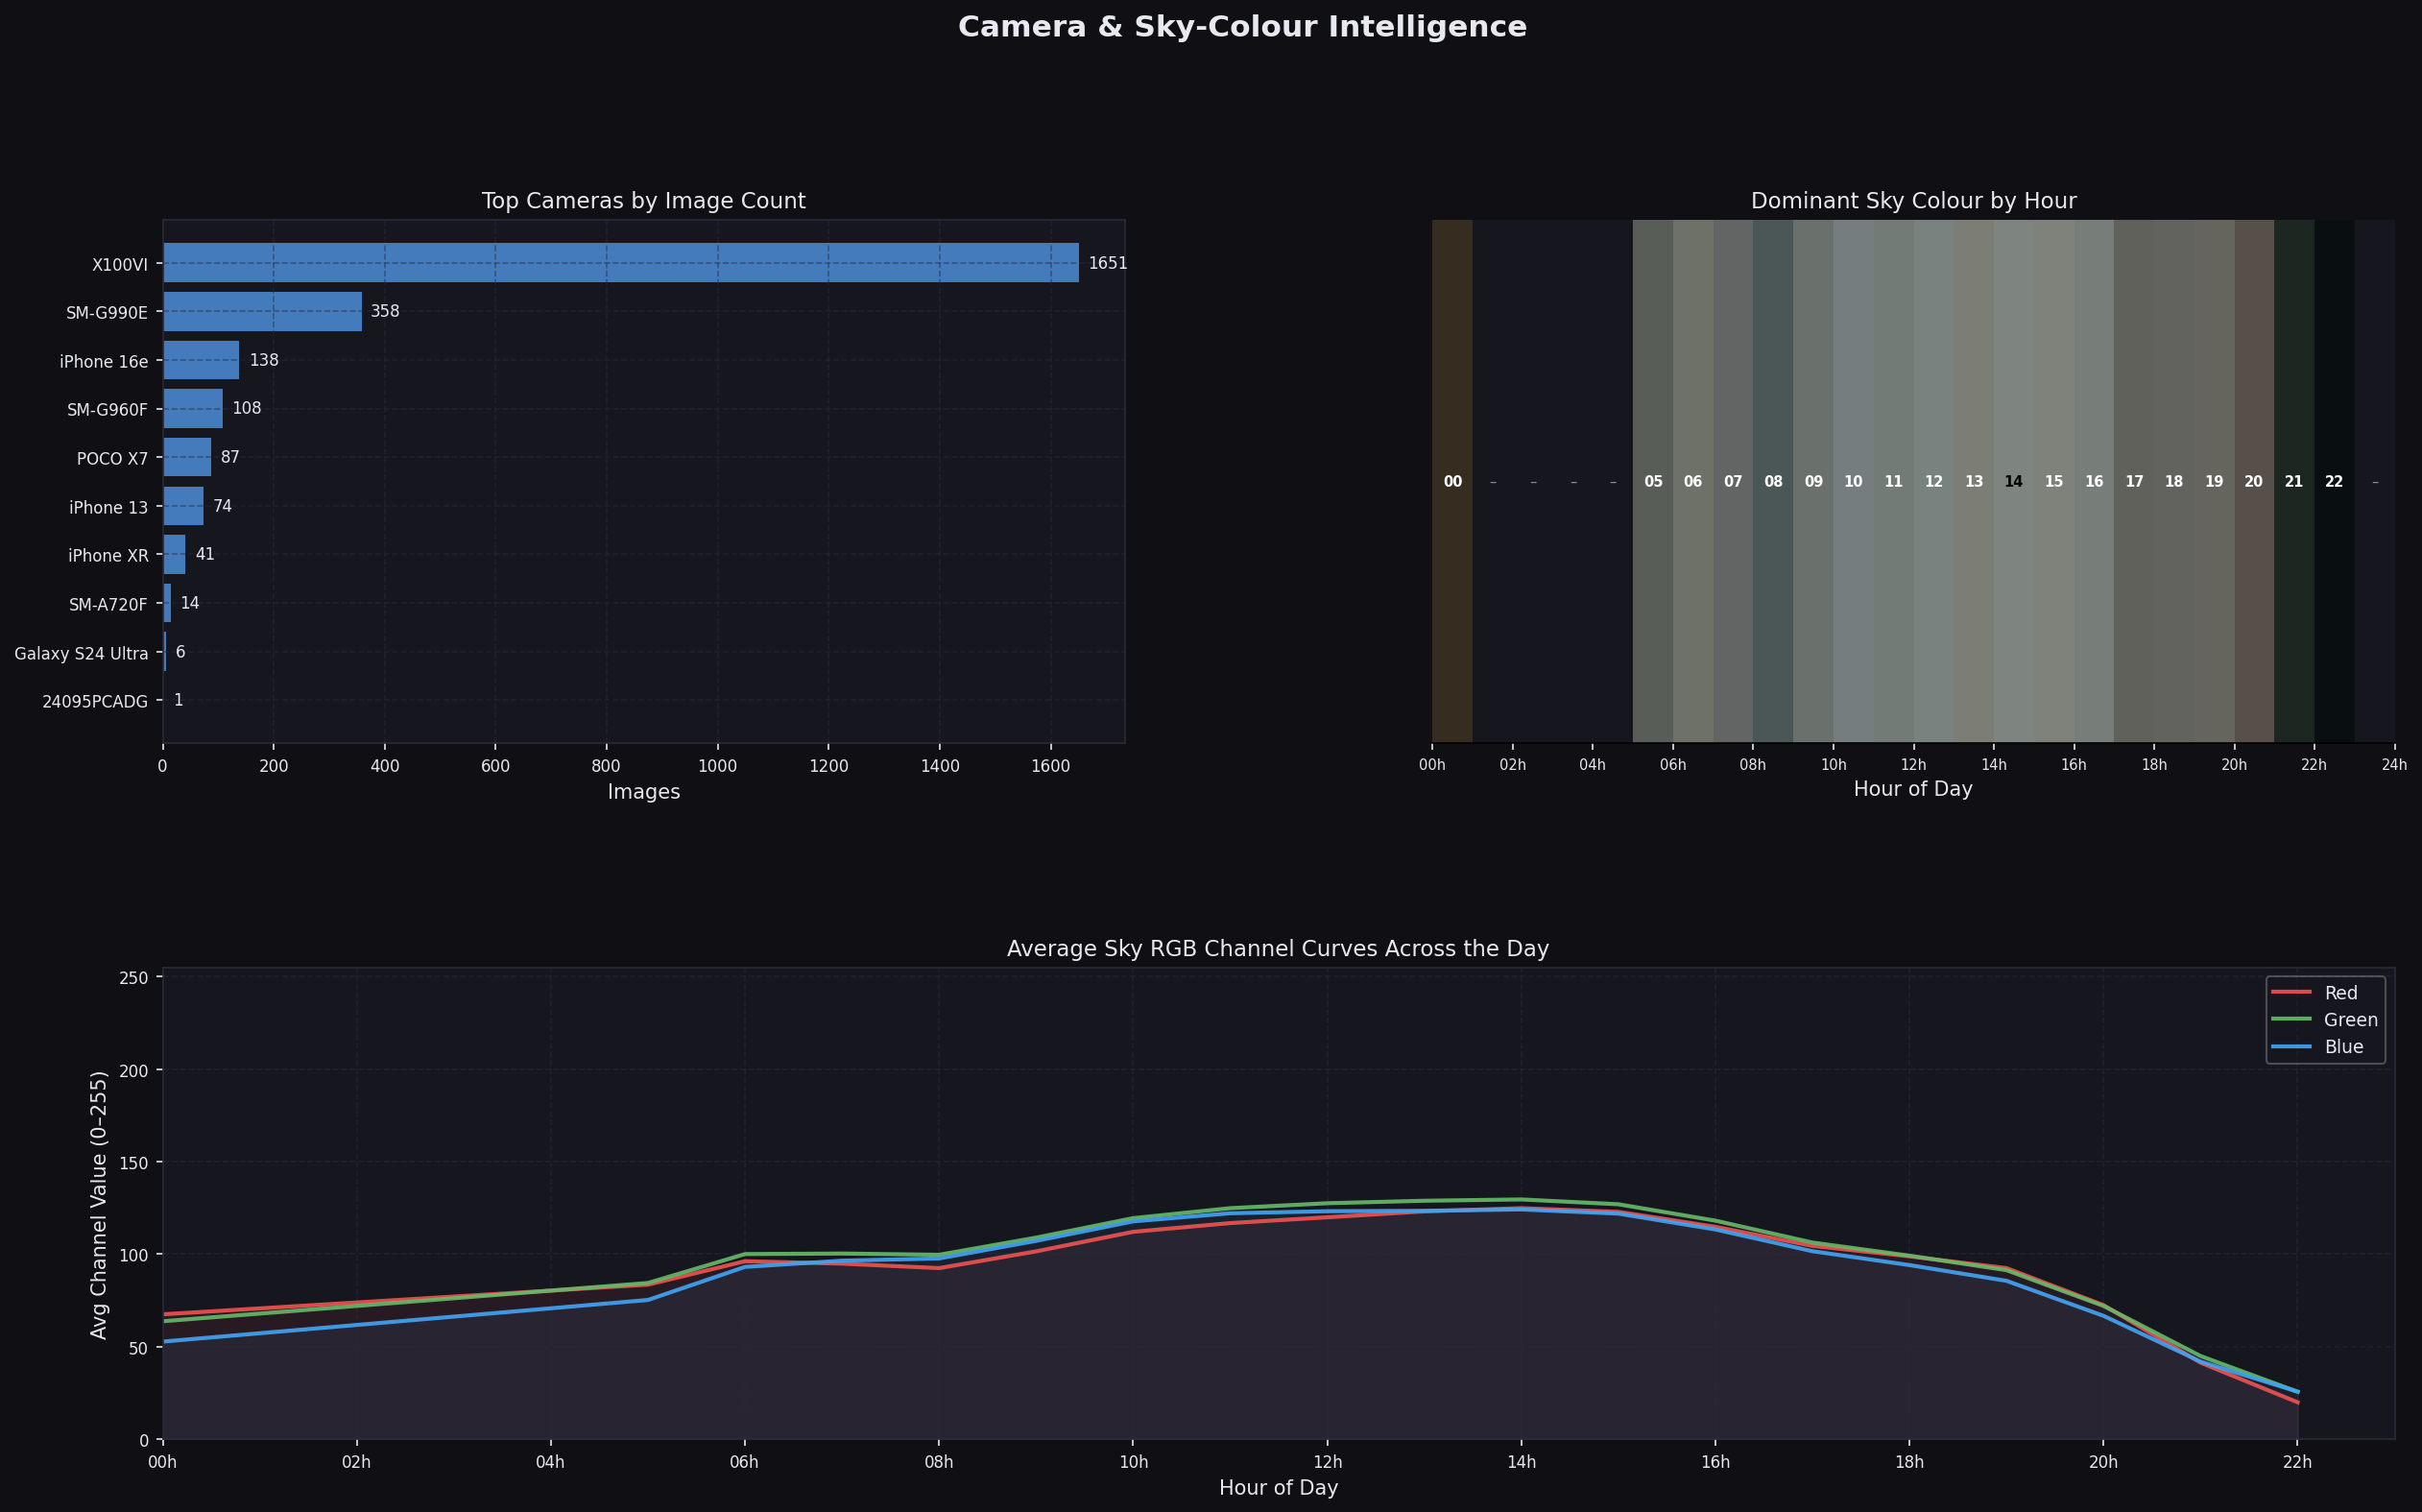
\includegraphics[width=0.75\linewidth]{dataset_report_p3_colour.png}
  \caption{Color temperature and channel statistics distribution across the dataset.}
  \label{fig:dataset_colour}
\end{figure}

\begin{figure}[H]
  \centering
  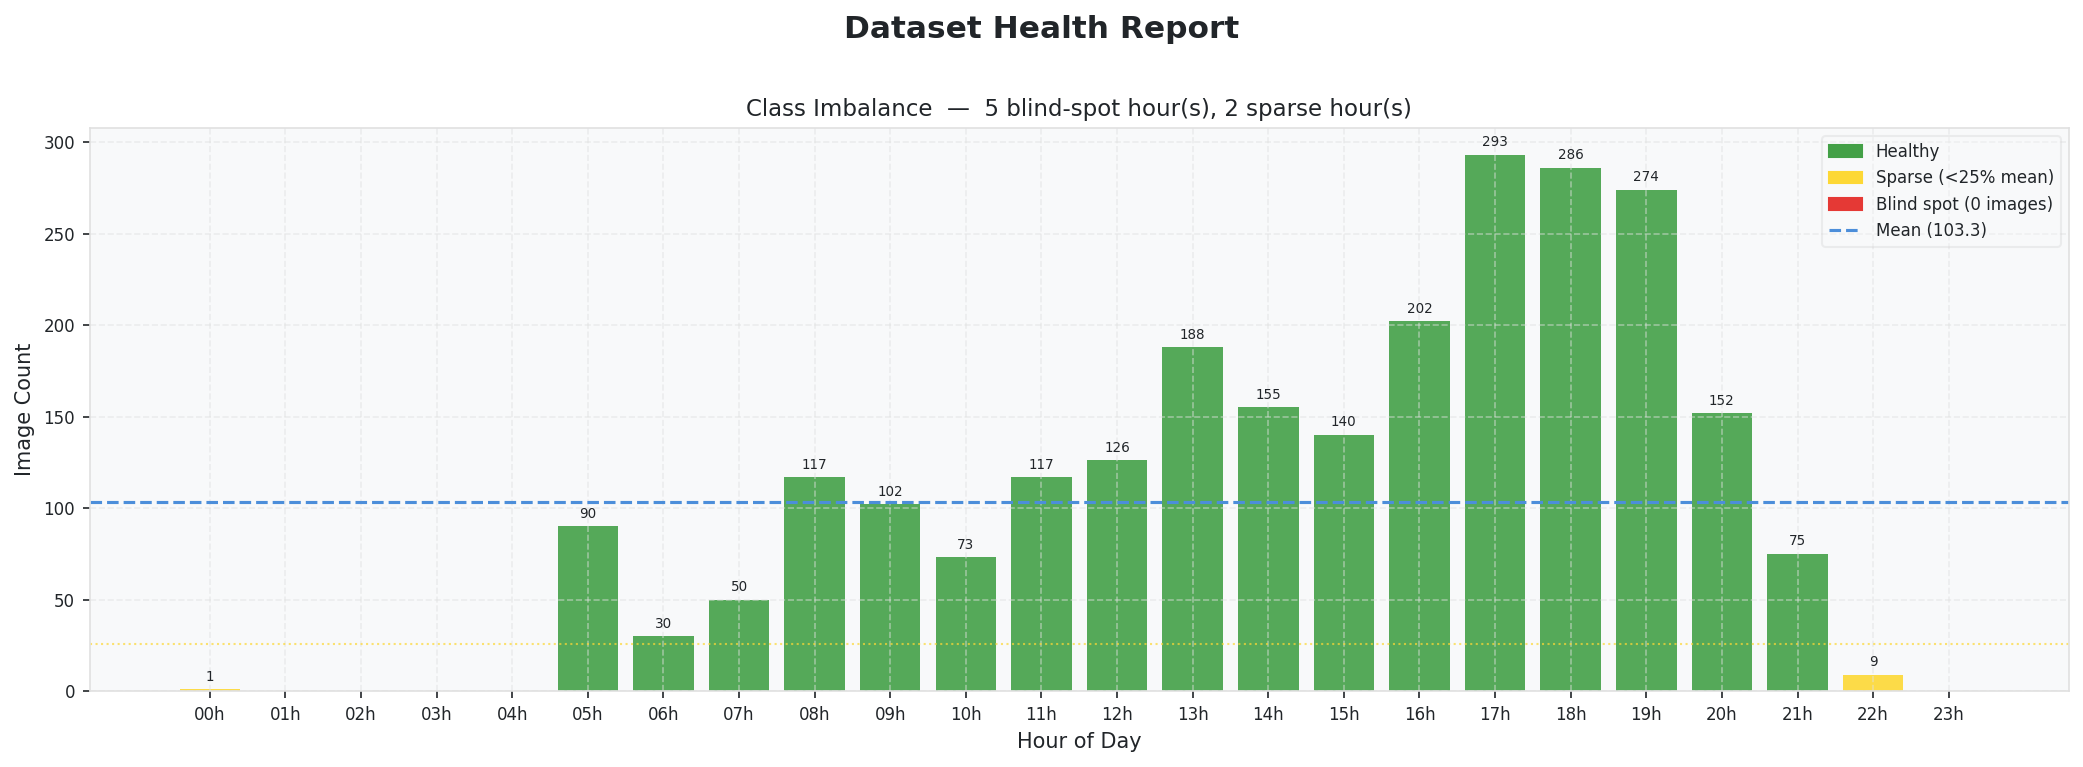
\includegraphics[width=0.75\linewidth]{dataset_report_p4_health.png}
  \caption{Dataset health report: exposure balance and label density.}
  \label{fig:dataset_health}
\end{figure}

\subsection{Python Pipeline Parameters}

Hyperparameters were selected via Optuna over 15 Bayesian trials on a single fold. Table~\ref{tab:python_params} lists the final configuration.

\begin{table}[H]
\centering
\footnotesize
\caption{Python/PyTorch hyperparameters.}
\label{tab:python_params}
\begin{tabular}{lc}
\toprule
\textbf{Parameter} & \textbf{Value} \\
\midrule
Backbone            & ConvNeXt-Tiny \\
Frozen until        & \texttt{features.4} \\
MLP hidden dim      & 384 \\
Dropout             & 0.156 \\
Epochs              & 80 \\
Batch size          & 8 \\
Learning rate       & $4.42\times10^{-4}$ \\
LR minimum          & $1.83\times10^{-5}$ \\
Weight decay        & 0.0373 \\
Optimizer           & 8-bit AdamW \\
Schedule            & Cosine annealing \\
Mixup $\alpha$      & 0.178 \\
Label noise std     & 0.044 \\
\bottomrule
\end{tabular}
\end{table}

\subsection{MATLAB Pipeline Parameters}

Table~\ref{tab:matlab_params} lists the MATLAB training configuration. The CNN is trained for 30 epochs; the Random Forest and SVR use default MATLAB settings with the parameters below.

\begin{table}[H]
\centering
\footnotesize
\caption{MATLAB pipeline parameters.}
\label{tab:matlab_params}
\begin{tabular}{lc}
\toprule
\textbf{Parameter} & \textbf{Value} \\
\midrule
Backbone            & SqueezeNet \\
Frozen layers       & fire1--fire6 \\
Epochs              & 30 \\
Optimizer           & Adam \\
Initial LR          & $10^{-3}$ \\
Dropout             & 0.4 \\
Date branch dim     & 64 \\
Classical feat.\ dim & 145 \\
RF trees            & 100 \\
SVR kernel          & RBF \\
\bottomrule
\end{tabular}
\end{table}

% ========================================================================
%  4. RESULTS
% ========================================================================
\section{Results}

\subsection{Python Pipeline Results}

Table~\ref{tab:python_results} reports the per-fold validation MAE for the ConvNeXt-based model. The best fold achieves 49.38 min MAE at epoch 62 and the mean across all five folds is 54.61 min.

\begin{table}[H]
\centering
\footnotesize
\caption{Python ConvNeXt: per-fold validation MAE.}
\label{tab:python_results}
\begin{tabular}{lcc}
\toprule
\textbf{Fold} & \textbf{Best Epoch} & \textbf{Val MAE (min)} \\
\midrule
1 & 62 & 49.38 \\
2 & 73 & 53.93 \\
3 & 66 & 54.75 \\
4 & 79 & 54.83 \\
5 & 79 & 60.18 \\
\midrule
\textbf{Mean} & & \textbf{54.61} \\
\bottomrule
\end{tabular}
\end{table}

Figure~\ref{fig:python_training} shows the training curves for the Python pipeline.

\begin{figure}[H]
  \centering
  
\includegraphics[width=0.75\linewidth]{training_report.png}
  \caption{Training loss and validation MAE curves for the Python ConvNeXt pipeline across all five folds.}
  \label{fig:python_training}
\end{figure}

The model converges consistently across folds. Best checkpoints occur at late epochs (62--79), which is expected from the cosine annealing schedule that refines weights at low learning rates. Fold 5 shows slightly higher error (60.18 min), likely due to an unfavorable data split covering fewer twilight examples.

\subsection{MATLAB Pipeline Results}

Table~\ref{tab:matlab_results} presents the test MAE per fold for the MATLAB SqueezeNet CNN, together with the final training and validation RMSE in fractional hours as recorded in the convergence logs.

\begin{table}[H]
\centering
\footnotesize
\caption{MATLAB SqueezeNet CNN: per-fold results.}
\label{tab:matlab_results}
\begin{tabular}{lccc}
\toprule
\textbf{Fold} & \textbf{Tr.RMSE (h)} & \textbf{Val.RMSE (h)} & \textbf{MAE (min)} \\
\midrule
1 & 0.338 & 0.560 & 87.59 \\
2 & 0.292 & 0.562 & 82.86 \\
3 & 0.271 & 0.545 & 82.11 \\
4 & 0.290 & 0.549 & 74.22 \\
5 & 0.266 & 0.560 & 79.02 \\
\midrule
\textbf{Mean} & & & \textbf{81.16} \\
\bottomrule
\end{tabular}
\end{table}

Figure~\ref{fig:matlab_convergence} shows the MATLAB convergence curves.

\begin{figure}[H]
  \centering
  
\includegraphics[width=0.75\linewidth]{matlab_convergence.png}
  \caption{MATLAB SqueezeNet CNN: training and validation RMSE per epoch across all five folds.}
  \label{fig:matlab_convergence}
\end{figure}

The MATLAB CNN converges from an initial RMSE of approximately 1.0--1.3 h to below 0.60 h within the first 10 epochs across all five folds.

\subsection{Comparative Analysis}

Table~\ref{tab:comparison} presents a direct comparison of both pipelines. The Python ConvNeXt model outperforms the MATLAB SqueezeNet CNN by 26.55 min MAE (32.7\% relative improvement). This gap is mainly due to the larger backbone capacity, higher input resolution ($512\times512$ vs $224\times224$), aggressive data augmentation, and Optuna-tuned hyperparameters. The MATLAB pipeline achieves competitive convergence in only 30 epochs, demonstrating that a lightweight model with cyclic date encoding is a viable baseline.

\begin{table}[H]
\centering
\footnotesize
\caption{Cross-pipeline comparison (5-fold mean MAE).}
\label{tab:comparison}
\resizebox{\columnwidth}{!}{%
\begin{tabular}{lcc}
\toprule
\textbf{Method} & \textbf{Resolution} & \textbf{MAE (min)} \\
\midrule
SqueezeNet CNN (MATLAB) & $224\times224$ & 81.16 \\
ConvNeXt-Tiny + MLP (Python) & $512\times512$ & \textbf{54.61} \\
\bottomrule
\end{tabular}%
}
\end{table}

\begin{figure}[H]
  \centering
  
\includegraphics[width=0.75\linewidth]{comparison_barchart.png}
  \caption{Mean Absolute Error (MAE) comparison across folds between the Python and MATLAB pipelines.}
  \label{fig:comparison_barchart}
\end{figure}

Sample prediction visualizations from the Python pipeline are shown in Figure~\ref{fig:visualizations}.

\begin{figure}[H]
  \centering
  
\includegraphics[width=0.75\linewidth]{predictions.png}
  \caption{Predicted vs actual time-of-day for the Python ConvNeXt pipeline. Each point is a validation image coloured by cyclic error; the diagonal represents perfect prediction and the green band shows the $\pm$30-minute window.}
  \label{fig:visualizations}
\end{figure}

% ========================================================================
%  5. CONCLUSIONS
% ========================================================================
\section{Conclusions}

This paper presented a comprehensive framework for estimating the time of day from single sky photographs by fusing deep convolutional features with handcrafted photometric descriptors and cyclically encoded calendar metadata. The proposed methodology addresses the fundamental limitations of brightness-based heuristics used in conventional image organization systems by incorporating multi-modal cues---color temperature, sky gradients, edge density, seasonal solar positioning, and geographic coordinates---into a unified regression pipeline.

The cyclic sine--cosine encoding scheme for both the target variable and temporal metadata features proved essential for modeling the circular nature of the 24-hour clock and the annual calendar cycle, eliminating artificial discontinuities that would otherwise degrade regression performance. The integration of 77-dimensional handcrafted features alongside the ConvNeXt-Tiny backbone's learned representations provided complementary information channels that enhanced estimation accuracy beyond what either modality could achieve independently.

The dual-pipeline implementation---a primary Python/PyTorch system and a parallel MATLAB-based system with classical baselines---enabled a meaningful comparative analysis between modern deep learning approaches and established machine learning techniques for this regression task. The Optuna-driven hyperparameter optimization ensured that the reported configurations represent near-optimal operating points for the given dataset and architecture.

Future work may extend this framework in several directions: incorporating attention mechanisms to automatically identify informative image regions, leveraging sun position estimation from shadow analysis as an auxiliary prediction target, expanding the dataset to include diverse geographic locations and climatic conditions to improve generalization, and deploying the trained model as a lightweight mobile application for real-time image metadata correction.

% ========================================================================
%  REFERENCES
% ========================================================================
\section*{References}
\begin{sloppypar}
\begin{enumerate}[label={[\arabic*]}, leftmargin=*, itemsep=2pt, parsep=0pt, font=\small]

\item Lalonde, J.-F., Efros, A.A., Narasimhan, S.G. 2012. Estimating the Natural Illumination Conditions from a Single Outdoor Image. \textit{International Journal of Computer Vision}, 98(2), pp.~123--145. DOI: 10.1007/s11263-011-0501-8

\item Hold-Geoffroy, Y., Sunkavalli, K., Hadap, S., Gambaretto, E., Lalonde, J.-F. 2017. Deep Outdoor Illumination Estimation. \textit{Proc.\ IEEE CVPR}, pp.~7312--7321. DOI: 10.1109/CVPR.2017.774

\item Wu, L., Ganesh, A., Shi, B., Matsushita, Y., Wang, Y., Ma, Y. 2010. Robust Photometric Stereo via Low-Rank Matrix Completion and Recovery. \textit{Proc.\ 10th Asian Conference on Computer Vision (ACCV)}, pp.~703--717. DOI: 10.1007/978-3-642-19318-7\_55

\item Liu, Z., Mao, H., Wu, C.-Y., Feichtenhofer, C., Darrell, T., Xie, S. 2022. A ConvNet for the 2020s. \textit{Proc.\ IEEE/CVF CVPR}, pp.~11976--11986. DOI: 10.1109/CVPR52688.2022.01167

\item Dettmers, T., Lewis, M., Belkada, Y., Zettlemoyer, L. 2022. 8-bit Optimizers via Block-wise Quantization. \textit{Proc.\ ICLR}. arXiv:2110.02861

\item Akiba, T., Sano, S., Yanase, T., Ohta, T., Koyama, M. 2019. Optuna: A Next-generation Hyperparameter Optimization Framework. \textit{Proc.\ ACM SIGKDD}, pp.~2623--2631. DOI: 10.1145/3292500.3330701

\item Russakovsky, O., et al. 2015. ImageNet Large Scale Visual Recognition Challenge. \textit{International Journal of Computer Vision}, 115(3), pp.~211--252. DOI: 10.1007/s11263-015-0816-y

\item Krizhevsky, A., Sutskever, I., Hinton, G.E. 2012. ImageNet Classification with Deep Convolutional Neural Networks. \textit{Advances in Neural Information Processing Systems (NeurIPS)}, 25, pp.~1097--1105.

\item Canny, J. 1986. A Computational Approach to Edge Detection. \textit{IEEE Transactions on Pattern Analysis and Machine Intelligence}, 8(6), pp.~679--698. DOI: 10.1109/TPAMI.1986.4767851

\item Cubuk, E.D., Zoph, B., Shlens, J., Le, Q.V. 2020. Randaugment: Practical Automated Data Augmentation with a Reduced Search Space. \textit{Proc.\ IEEE CVPR Workshops}, pp.~702--703. DOI: 10.1109/CVPRW50498.2020.00359

\item Zhong, Z., Zheng, L., Kang, G., Li, S., Yang, Y. 2020. Random Erasing Data Augmentation. \textit{Proc.\ AAAI Conference on Artificial Intelligence}, 34(7), pp.~13001--13008. DOI: 10.1609/aaai.v34i07.7000

\item Zhang, H., Cisse, M., Dauphin, Y.N., Lopez-Paz, D. 2018. mixup: Beyond Empirical Risk Minimization. \textit{Proc.\ International Conference on Learning Representations (ICLR)}.

\item Loshchilov, I., Hutter, F. 2019. Decoupled Weight Decay Regularization. \textit{Proc.\ ICLR}.

\item Loshchilov, I., Hutter, F. 2017. SGDR: Stochastic Gradient Descent with Warm Restarts. \textit{Proc.\ ICLR}.

\item Buda, M., Maki, A., Mazurowski, M.A. 2018. A Systematic Study of the Class Imbalance Problem in Convolutional Neural Networks. \textit{Neural Networks}, 106, pp.~249--259. DOI: 10.1016/j.neunet.2018.07.011

\item Zhou, Z.-H. 2012. Ensemble Methods: Foundations and Algorithms. CRC Press.

\item Iandola, F.N., Han, S., Moskewicz, M.W., Ashraf, K., Dally, W.J., Keutzer, K. 2016. SqueezeNet: AlexNet-level accuracy with 50x fewer parameters and less than 0.5MB model size. arXiv:1602.07360.

\item Breiman, L. 2001. Random Forests. \textit{Machine Learning}, 45(1), pp.~5--32. DOI: 10.1023/A:1010933404324

\item Smola, A.J., Scholkopf, B. 2004. A Tutorial on Support Vector Regression. \textit{Statistics and Computing}, 14(3), pp.~199--222. DOI: 10.1023/B:STCO.0000035301.49549.88

\item Arlot, S., Celisse, A. 2010. A Survey of Cross-Validation Procedures for Model Selection. \textit{Statistics Surveys}, 4, pp.~40--79. DOI: 10.1214/09-SS054

\end{enumerate}
\end{sloppypar}

\end{document}
